\documentclass[../main.tex]{subfiles}
\begin{document}

\section{Hypothesis Testing for a Single Sample}
The values contained within a two-sided level $100(1-\alpha)\%$ confidence intervals are precisely those values for which the P-value of a two-tailed hypothesis test will be greater than $\alpha$.

\subsection{Large sample tests for a population mean}
The \textbf{null hypothesis} says that the effect indicated by the sample is due only to random variation between the sample and the population, denote by $H_0$.\\
Null hypothesis has a form of $H_0:\mu\leq\mu_0$ or $H_0:\mu\geq\mu_0$ or $H_0:\mu=\mu_0$\\
\\
The \textbf{alternative hypothesis} says that the effect indicated by the sample is real, in that accurately represents the whole population, denote by $H_1$.\\
\\
Steps for a Hypothesis Test:\\
1. Define the null hypothesis \hn and the alternate hypothesis \ha.\\
2. Assume \hn to be true.\\
3. Compute a test statistic.\\
4. Compute the P-value\\
5. State a conclution about the strength of the evidence against \hn.

\subsection{Draw conclusions from the results of hypothesis tests}
Only two conclusions can be reached:\\
1. we reject \hn / we conclude that \hn is false. (Smaller P-value)\\
2. we do not reject \hn . / \hn is plausible. (Larger P-value) \\
Note: we can never conclude that \hn is true. \\
We must decide whether the level of disagreement, measured with the P value, is great enough to render the null hypothesis implausible.
Reject \hn whenever $P\leq 0.05$.

\subsection{Z score, Z table, p value}
\subsubsection*{P-value}
The \textbf{P-value} is the probability, assuming \hn to be true, that the test statistic would have a value whose disagreement with \hn is as great as or greater than what was actually observed. The P value is also called the \textbf{observed significance level}\\
The P-value measures the plausibility of $H_0$. The smaller P-value , the stronger rejecting $H_0$.\\
If the P-value is sufficiently small, we could reject our assumption that $H_0$ is true. \\
\\
The P-value is an area under the normal curve, which depends on the alternate hypothesis as follows:\\
1. If $H_1:\mu>\mu_0$,P-value is the area to the right of z.\\
2. If $H_1:\mu<\mu_0$,P-value is the area to the left of z.\\
3. If $H_1:\mu\neq\mu_0$,P-value is the sum of the areas in the tails cut off by z and -z.\\
\\
If $P\leq 0.05$, the result is statistically significant at the 5\% level. And, if $P\leq 0.01$, the result is statistically significant at the 1\% level.\\
\\
\subsubsection*{z-score}
\[z = \frac{\xbar - \mu _0 }{\sigma/{\sqrt{n}}}\]
If $\sigma$ is unknown, it may be approximated by s.

\subsection{Tests for a population proportion and differences in two proportions}
A population proportion is simply a population mean for a population of 0s and 1s: a Bernoulli population.\\
Let X be the number of successes in n independent Bernoulli trails, each with success probability p.
$$X\sim Bin(n,p)$$
The sample proportion will be approximately normally distributed whenever both $n p_0 >10$ and $n(1-p_0)>10$, where $p_0$ is the population proportion specified in the null distribution.\\
To test a null hypothesis in the form:$H_0:p\leq p_0$ or $H_0:p \geq p_0$ or $H_0: p=p_0$, compute z-score:
\[z = \frac{\phat - p_0 }{\sqrt{\frac{p_0 (1-p_0)}{n}}}\]

\subsection{Small-sample tests for a population mean}
Let \xotn be a sample from a normal population with mean $\mu$ and standard deviation $\sigma$ unknown.
To test a null hypothesis has a form of $H_0:\mu\leq\mu_0$ or $H_0:\mu\geq\mu_0$ or $H_0:\mu=\mu_0$\\
\[t= \frac{\xbar - \mu_0}{s/{\sqrt{n}}}\]
If $\sigma$ is known, use the z table and perform a z test.

\subsection{The Chi-Square Test}
A generalization of the Bernoulli trial is the multinomial trial, which is an experiment that can result in any one of k outcomes, where $k \geq 2$. The probabilities of the k outcomes are denoted \potk.\\
The results obtained are called observed values.\\
\\
Let k be the number of possible outcomes and let $O_i$ and $E_i$ be the observed and expected number of trials that result in outcome i.\\
The \textbf{chi square statistic} is:
\begin{equation*}
    \chi ^2 = \sum_{i=1}^{k} \frac{(O_i - E_i)^2}{E_i}
\end{equation*}
The larger the $\chi ^2$, the stronger the evidence against $H_0$.\\
When the expected values are all sufficiently large, a good approximation is available. It is called the \textbf{chi-square distribution} with $k-1$ degrees of freedom.\\
Use of the chi square distribution is appropriate whenever all the expected values $\geq$ 5.
Chi-square test determines how well a given multinomial distribution fits the data. For this reason it is called a \textbf{goodness of fit test}.

\subsubsection*{Test for Homogeneity}
The null hypothesis is that the probabilities of the outcomes are the same for each experiment.\\
\\
The \textbf{contingency table}: The number in the cell at the intersection of row i and column j is the number of trials whose outcome was observed to fall into row category i and into column category j . This number is called the \textbf{observed value} for cell ij .\\
\\
The total of observed values for each row and column are called \textbf{marginal totals}.\\
Let I denote the number of rows in the table.\\
Let J denote the number of columns. \\
Let $p_{ij}$ denote the probability that the outcome of a trial falls into column j given that it is in row i.\\ 
Then the null hypothesis: $H_0$ for each column j, $p_{1j}=...=p_{Ij}$\\
Let $O_{ij}$ denote the observed value in cell ij.\\
Let $O..$ denote the sum of the observed values in all the cells.\\
The expected count:\[
E_{ij}=\frac{O_{i.}O_{.j}}{O_{..}}\]
\begin{equation*}
    \chi ^2 = \sum_{i=1}^{I} \sum_{j=1}^{J} \frac{(O_i - E_i)^2}{E_i}
\end{equation*}

\subsection{Fixed-level testing}
If a decision is going to be made on the basis of a hypothesis test, there is no choice but to pick a cut off point for the P value. When this is done, the test is referred to as a \textbf{fixed level test}.\\\\
A value $\alpha$ is called the \textbf{significant level} of the test, where $0<\alpha < 1$ is chosen. The P-value is computed. \\
If $P\leq\alpha$, the null hypothesis is rejected, the alternate hypothesis is taken as truth.\\
If $P>\alpha$, the null hypothesis is considered to be plausible.\\
\\
In fixed-level test, a critical point is the test statistic that produces a P-value exactly = $\alpha$.\\
If the test statistic is on one side of the critical point, the P-value $<\alpha$, and \hn will be rejected.\\
If the test statistic is on the other side of the critical point, P-value $>\alpha$, and \hn will not be rejected.\\
The region on the side of the critical point that leads to rejection is called the \textbf{rejection region}. The critical point is in the region.

\subsection{Power}
The power of the test is the probability of rejecting \hn when it is false.
$$\mbox{Power} = 1-P(\mbox{Type II Error})$$
To be useful, a test must have reasonably small probabilities of both type I and type II errors.\\
The type I error is kept small by choosing a small value of $\alpha$ as the significance level. Then the power of the test is calculated. If the power is large, then the probability of a type II error is small as well, and the test is a useful one.\\
\\
Computing the power involves two steps:\\
1. Compute the rejection region.\\
2. Compute the probability that the test statistic falls in the rejection region if the alternate hypothesis is true. This is the power.\\
\\
In general, tests with power greater than 0.80 or perhaps 0.90 are considered acceptable, but there are no well

\subsection{Multiple tests}
When \hn is rejected, we have strong evidence that it is false. But strong evidence is not certainty.\\
Occasionally, a true null hypothesis will be rejected. When many tests are performed, it is more likely that some true null hypotheses will be rejected. Thus when many tests are performed, it is difficult to tell which of the rejected null hypotheses are really false and which correspond to type I errors.

\subsubsection*{The Bonferroni Method}
The Bonferroni method provides a way to adjust P values upward when several hypothesis tests are performed.\\
If a P value remains small after the adjustment, the null hypothesis may be rejected.\\
To make the Bonferroni adjustment, simply multiply the P value by the number of test performed.
\newpage
\subsection*{Type of Error}
Type I error: Reject \hn when it is true.\\
Type II error: Fail to reject \hn when it is false.
\begin{figure}[bh]
\centering
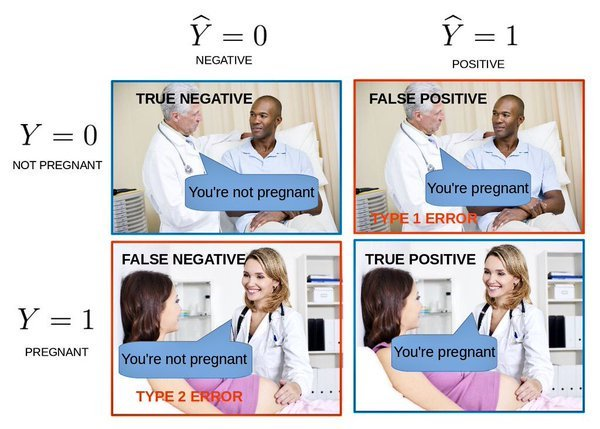
\includegraphics[width=15cm]{Sections/Image/TypeError.jpeg}
\caption{Type of Errors}
\end{figure}

\end{document}